\newif\iffunny
\funnyfalse

\documentclass[xcolor={dvipsnames}]{beamer}
\usepackage{color, colortbl}
\usepackage[ngerman,english]{babel}
\usepackage[T1]{fontenc}
\usepackage{CJKutf8} %japanese
\usepackage{lmodern}
%\usepackage{subfigure}
\usepackage[compatibility=false]{caption}
\usepackage{subcaption}
\usepackage{tikz}
\usepackage{textgreek}
\usepackage{tabularx}
\usepackage{booktabs}
\usepackage{siunitx}
\usepackage{units}
\usepackage{appendixnumberbeamer}
\usepackage[absolute,overlay]{textpos} %for positioning the logos where I want

\usepackage{animate}
\usepackage{multimedia}
\usepackage{fixltx2e}
\usepackage{multicol}
\usepackage{comment}
\DeclareSIUnit\year{yr}

\mode<presentation>
{
  \usetheme{CambridgeUS}     
  \usecolortheme{lily} 
  \definecolor{beamer@violet}{rgb}{0.5,0.3,0.5} % changed this
  \setbeamercolor{structure}{fg=beamer@violet!70!cyan}
  \setbeamercolor{palette primary}{fg=black, bg=gray!30!white!50!cyan!20!}
  \setbeamercolor{palette secondary}{fg=black, bg=gray!30!white!30!cyan!40!}
  \setbeamercolor*{palette tertiary}{bg=gray!20!white!20!cyan!60!}
  
  \setbeamercolor{frametitle}{fg=cyan!60!white!40!,bg=cyan!80!black}
  \setbeamercolor{title}{fg=cyan!80!black}
  \setbeamercolor{normal text}{fg=black,bg=white}
  \setbeamercolor{alerted text}{fg=beamer@violet}
  \setbeamercolor{example text}{fg=beamer@violet!70!cyan}
  
  \usefonttheme{structureitalicserif} 
  \setbeamertemplate{navigation symbols}{}
  \setbeamertemplate{caption}[numbered]
}
\newcommand{\sidlogo}{
  \setlength{\TPHorizModule}{1pt}
  \setlength{\TPVertModule}{1pt}
   % textblock{}{x,y}: pos(x) = rightUpperCorner + (x * \TPHorizModule), pos(y) = leftUpperCorner - (y * \TPVertModule)
  \begin{textblock}{1}(323,12)
   
\includegraphics[width=40pt,height=26pt]{figures/SiD.jpeg}
  \end{textblock}
  } 
\newcommand{\ilclogo}{
  \setlength{\TPHorizModule}{1pt}
  \setlength{\TPVertModule}{1pt}
   % textblock{}{x,y}: pos(x) = rightUpperCorner + (x * \TPHorizModule), pos(y) = leftUpperCorner - (y * \TPVertModule)
  \begin{textblock}{1}(323,12)
   
\includegraphics[width=40pt,height=26pt]{figures/ILC.jpeg}
  \end{textblock}
} 
\newcommand{\ejadelogo}{
  \setlength{\TPHorizModule}{1pt}
  \setlength{\TPVertModule}{1pt}
   % textblock{}{x,y}: pos(x) = rightUpperCorner + (x * \TPHorizModule), pos(y) = leftUpperCorner - (y * \TPVertModule)
  \begin{textblock}{1}(323,12)
   
\includegraphics[width=40pt,height=26pt]{figures/EJADE.jpeg}
  \end{textblock}
} 
\newcommand{\ATFlogo}{
  \setlength{\TPHorizModule}{1pt}
  \setlength{\TPVertModule}{1pt}
   % textblock{}{x,y}: pos(x) = rightUpperCorner + (x * \TPHorizModule), pos(y) = leftUpperCorner - (y * \TPVertModule)
  \begin{textblock}{1}(323,12)
   
\includegraphics[width=40pt,height=26pt]{figures/ATF_logo.jpg}
  \end{textblock}
} 
\newcommand{\RHULlogo}{
  \setlength{\TPHorizModule}{1pt}
  \setlength{\TPVertModule}{1pt}
   % textblock{}{x,y}: pos(x) = rightUpperCorner + (x * \TPHorizModule), pos(y) = leftUpperCorner - (y * \TPVertModule)
  \begin{textblock}{1}(337,12)
   
\includegraphics[width=25pt,height=26pt]{figures/rhul_logo.png}
  \end{textblock}
}
\newcommand{\flukalogo}{
  \setlength{\TPHorizModule}{1pt}
  \setlength{\TPVertModule}{1pt}
   % textblock{}{x,y}: pos(x) = rightUpperCorner + (x * \TPHorizModule), pos(y) = leftUpperCorner - (y * \TPVertModule)
  \begin{textblock}{1}(315,12)
   
\includegraphics[width=60pt,height=26pt]{figures/fluka_logo.png}
  \end{textblock}
} 

\newcommand{\electron}{e$^-$}
\newcommand{\positron}{e$^+$}

\title[ILC \& Background Simulations]{\textbf{\LARGE The International Linear Collider \\ \normalsize- \\ \small Background Simulations \& Optimizing the Final Focus Region}}
\author{\textbf{Anne Sch\"utz}\\
In collaboration with the SiD-Optimization group}
\institute{\textbf{KIT, DESY}}
\date[March 28th 2017]{\textbf{March 28th 2017}\\DPG 2017, M\"unster}

\titlegraphic{
\includegraphics[height=1.0cm]{figures/KIT.png}\hspace*{6cm}~%
   
\includegraphics[height=1.2cm]{figures/DESY_Logo.png}
}

\begin{document}

{
\usebackgroundtemplate{
 \tikz\node[opacity=0.1]{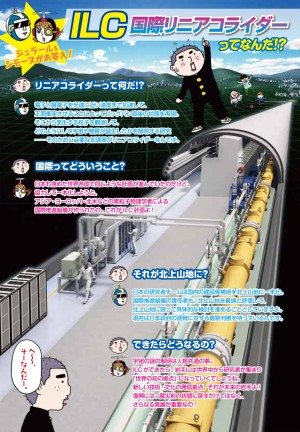
\includegraphics[width=\paperwidth]{figures/Iwatecomics.jpg}};
 % \tikz\node[opacity=0.2]{\centering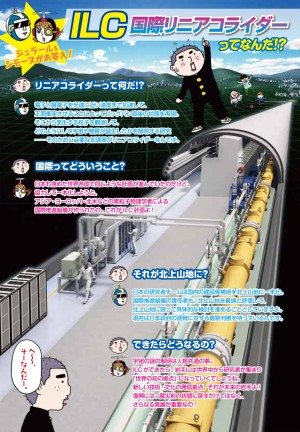
\includegraphics[height=\paperheight]{figures/Iwatecomics.jpg}};
 }
\begin{frame}
  \titlepage
\end{frame}
}

\begin{frame}{Table of contents}
  \tableofcontents
\end{frame}

\section{Physics motivation for a linear \positron \electron collider}

\begin{frame}{Comparison between ILC and LHC event displays}
\begin{center}
  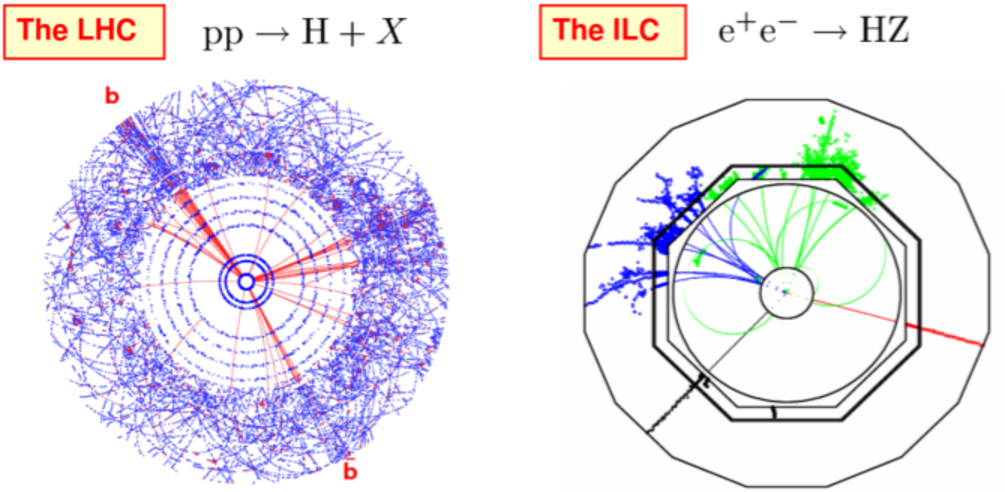
\includegraphics[width=0.75\textwidth]{figures/ILC_LHC_eventdisplay_comparison}
\end{center}
\end{frame}

\begin{frame}{The physics motivation in an overview}
\ilclogo
\visible<2->{ 
\alert{\MakeUppercase{Precision measurements:}}\\
}
\visible<3->{
\begin{itemize}
\item The \textbf{initial particle energy is precisely known}. There are no PDFs, as the initial particles are \textbf{elementary}.
\item Due to the \textbf{high energy resolution}, peaks are now measurable that weren't measurable before. Particles with small mass difference are distinguishable.
\item \textbf{c-tagging} is possible because of small distance between IP and the  detectors (nano-sized beam)
\end{itemize}
}
\visible<4->{ 
\alert{\MakeUppercase{Clean environment:}}\\
}
\visible<5->{
\begin{itemize}
\item \textbf{Small background}, and no underlying events or out-of-time pileup.
\end{itemize}
}
\visible<6->{
\alert{\MakeUppercase{Model independent:}}\\
}
\visible<7->{
\begin{itemize}
\item The events will be measured and reconstructed in completeness. \textbf{No theoretical assumptions} have to be taken into account.
\item \textbf{New physics and BSM physics}, which are not measurable at the LHC, are \textbf{accessible}.
\end{itemize}
}
\end{frame}


%-----------------------------------------------------------------------------
\AtBeginSection[]
{
  \begin{frame}<beamer>
     \tableofcontents[
     currentsection,
     hideothersubsections]
  \end{frame}
}

\section{The International Linear Collider}
\subsection{The layout}
\begin{frame}{The layout of the ILC}
\ilclogo
e$^+$e$^-$ linear collider:
\begin{itemize}
 \item \SI{30}{\kilo\metre} long
 \item adjustable center-of-mass energy
 \item polarized beams
 \item nanometer sized (!) beams at the IP
\end{itemize}
\begin{center}
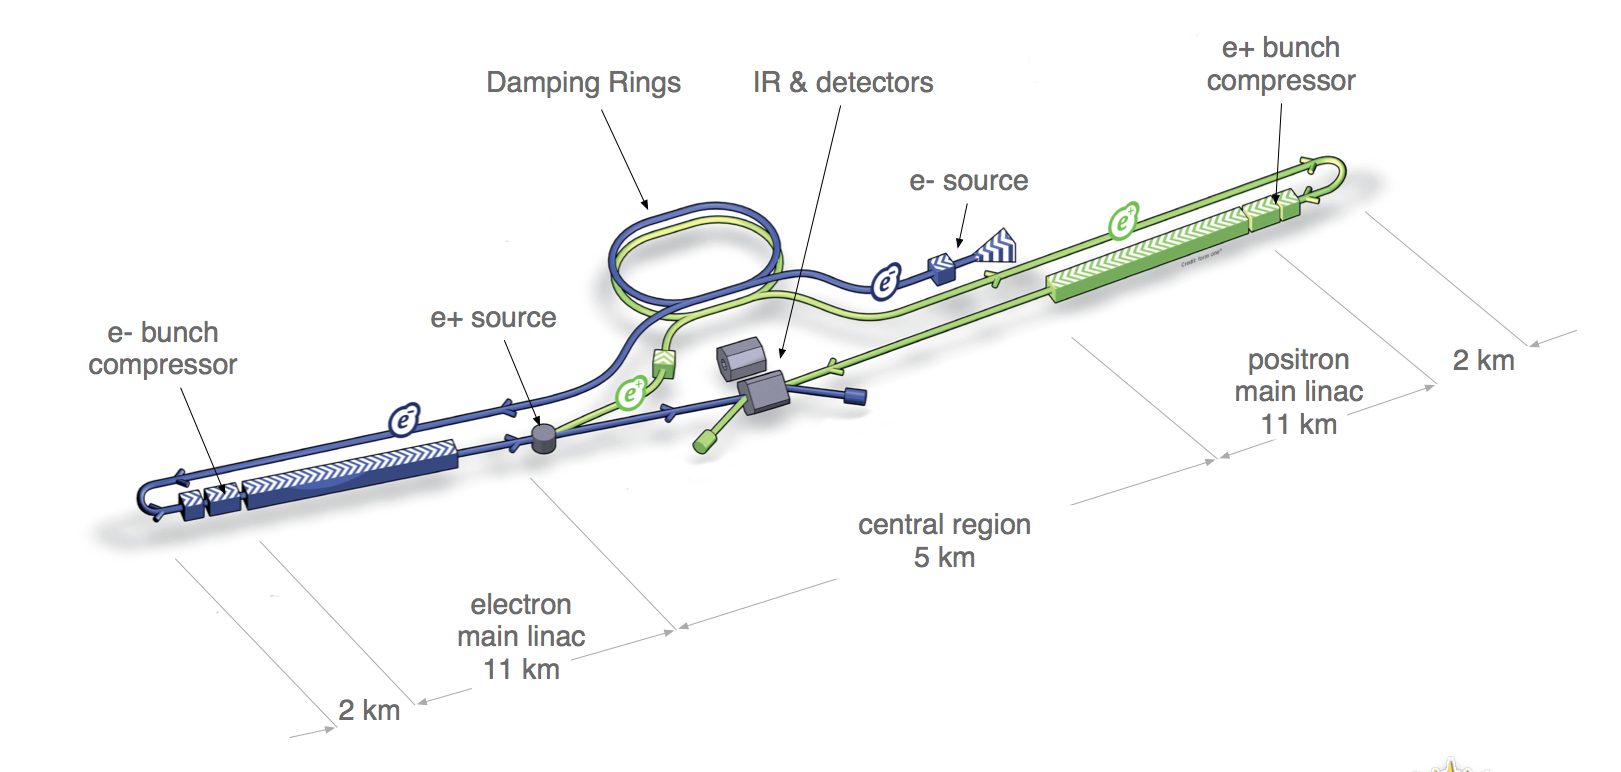
\includegraphics[width=\textwidth]{figures/ILC_schematic_layout.png}
\end{center}
\end{frame}

\subsection{The candidate site of the ILC}

\begin{frame}{The candidate site - The Kitakami mountains}
\ilclogo
\begin{center}
\begin{minipage}[t]{0.49\textwidth}
\centering
 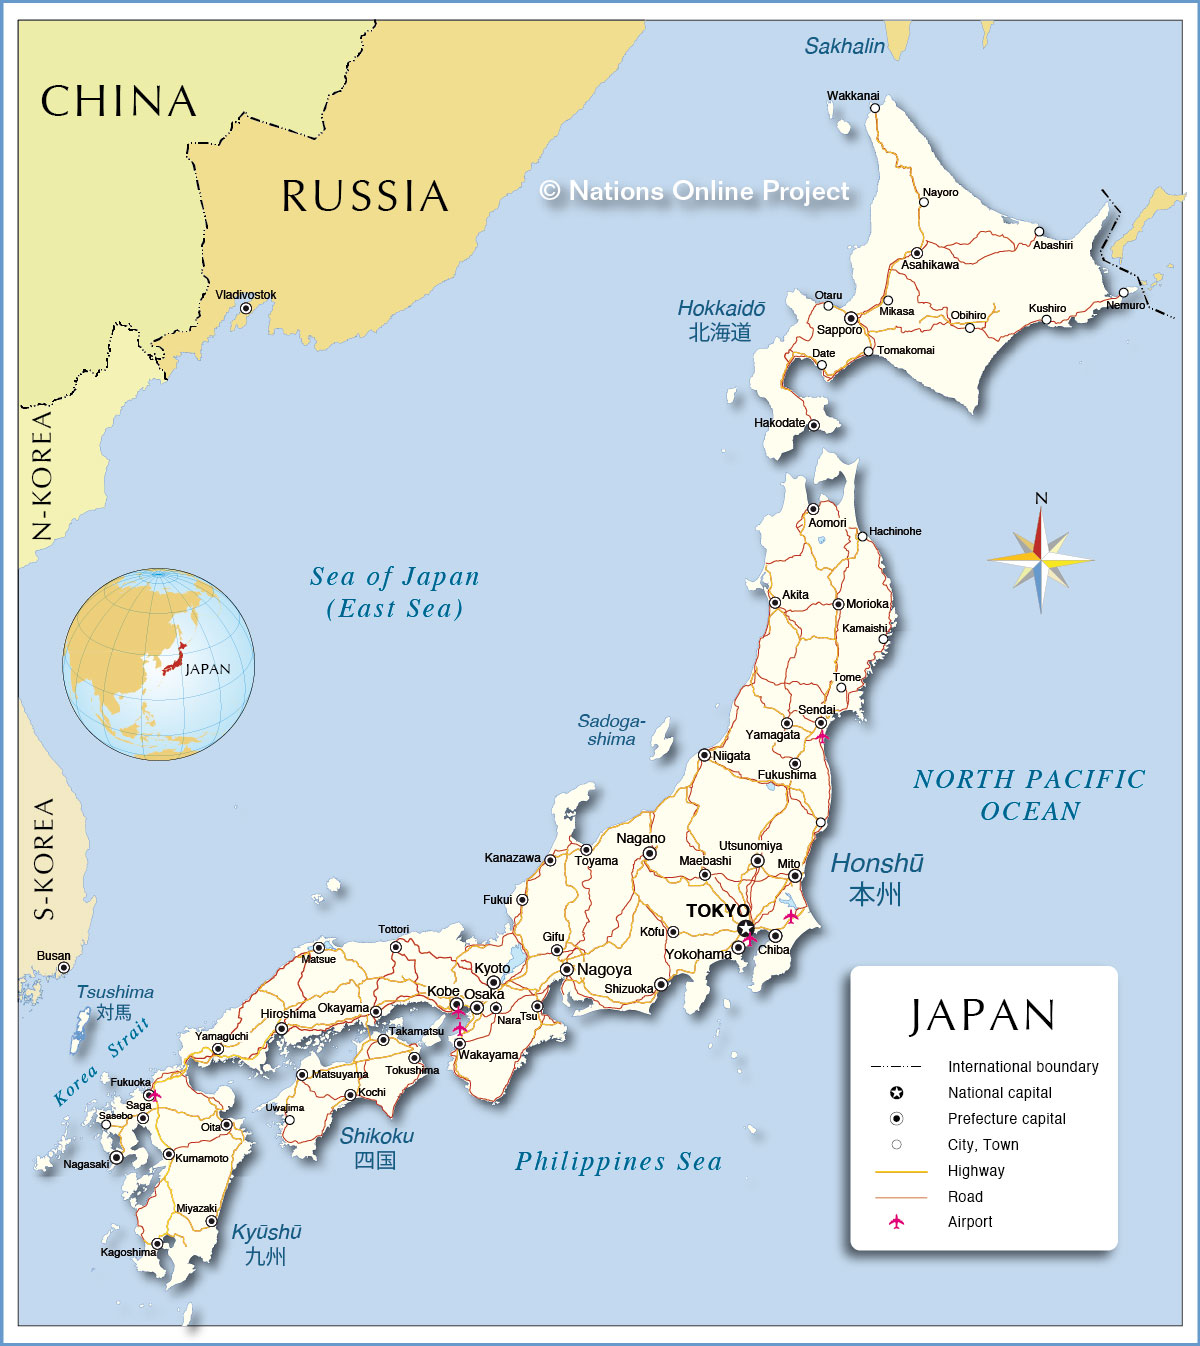
\includegraphics[width=\textwidth]{figures/japan-map.jpg}
\end{minipage}
\begin{minipage}[t]{0.48\textwidth}
\centering
   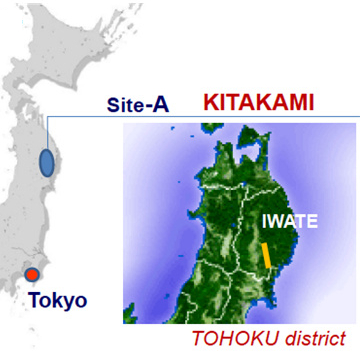
\includegraphics[width=\textwidth]{figures/Kitakami_site.jpg}
\end{minipage}
\begin{block}{}
 The ILC is under consideration by the Japanese government!
\end{block}

\end{center}
\end{frame}

\subsection{The detectors}
\begin{frame}{The two detectors - SiD and ILD}
\ilclogo
\begin{block}{}
The ILC has only one interaction point (IP)!\\
The two detectors can be swapped in the so-called \textbf{push-pull-system}.
\end{block}

\begin{columns}
\begin{column}{0.5\textwidth}
\begin{center}
\visible<2->{\alert{SiD - Silicon Detector}
\begin{itemize}
\item Height: $\sim$\SI{14}{\metre}, length:  $\sim$\SI{11}{\metre}
\item Weight: $\sim$\SI{10100}{\tonne}
\item Supercond. solenoid field: \SI{5}{\tesla}
\item Full silicon tracker
\end{itemize}
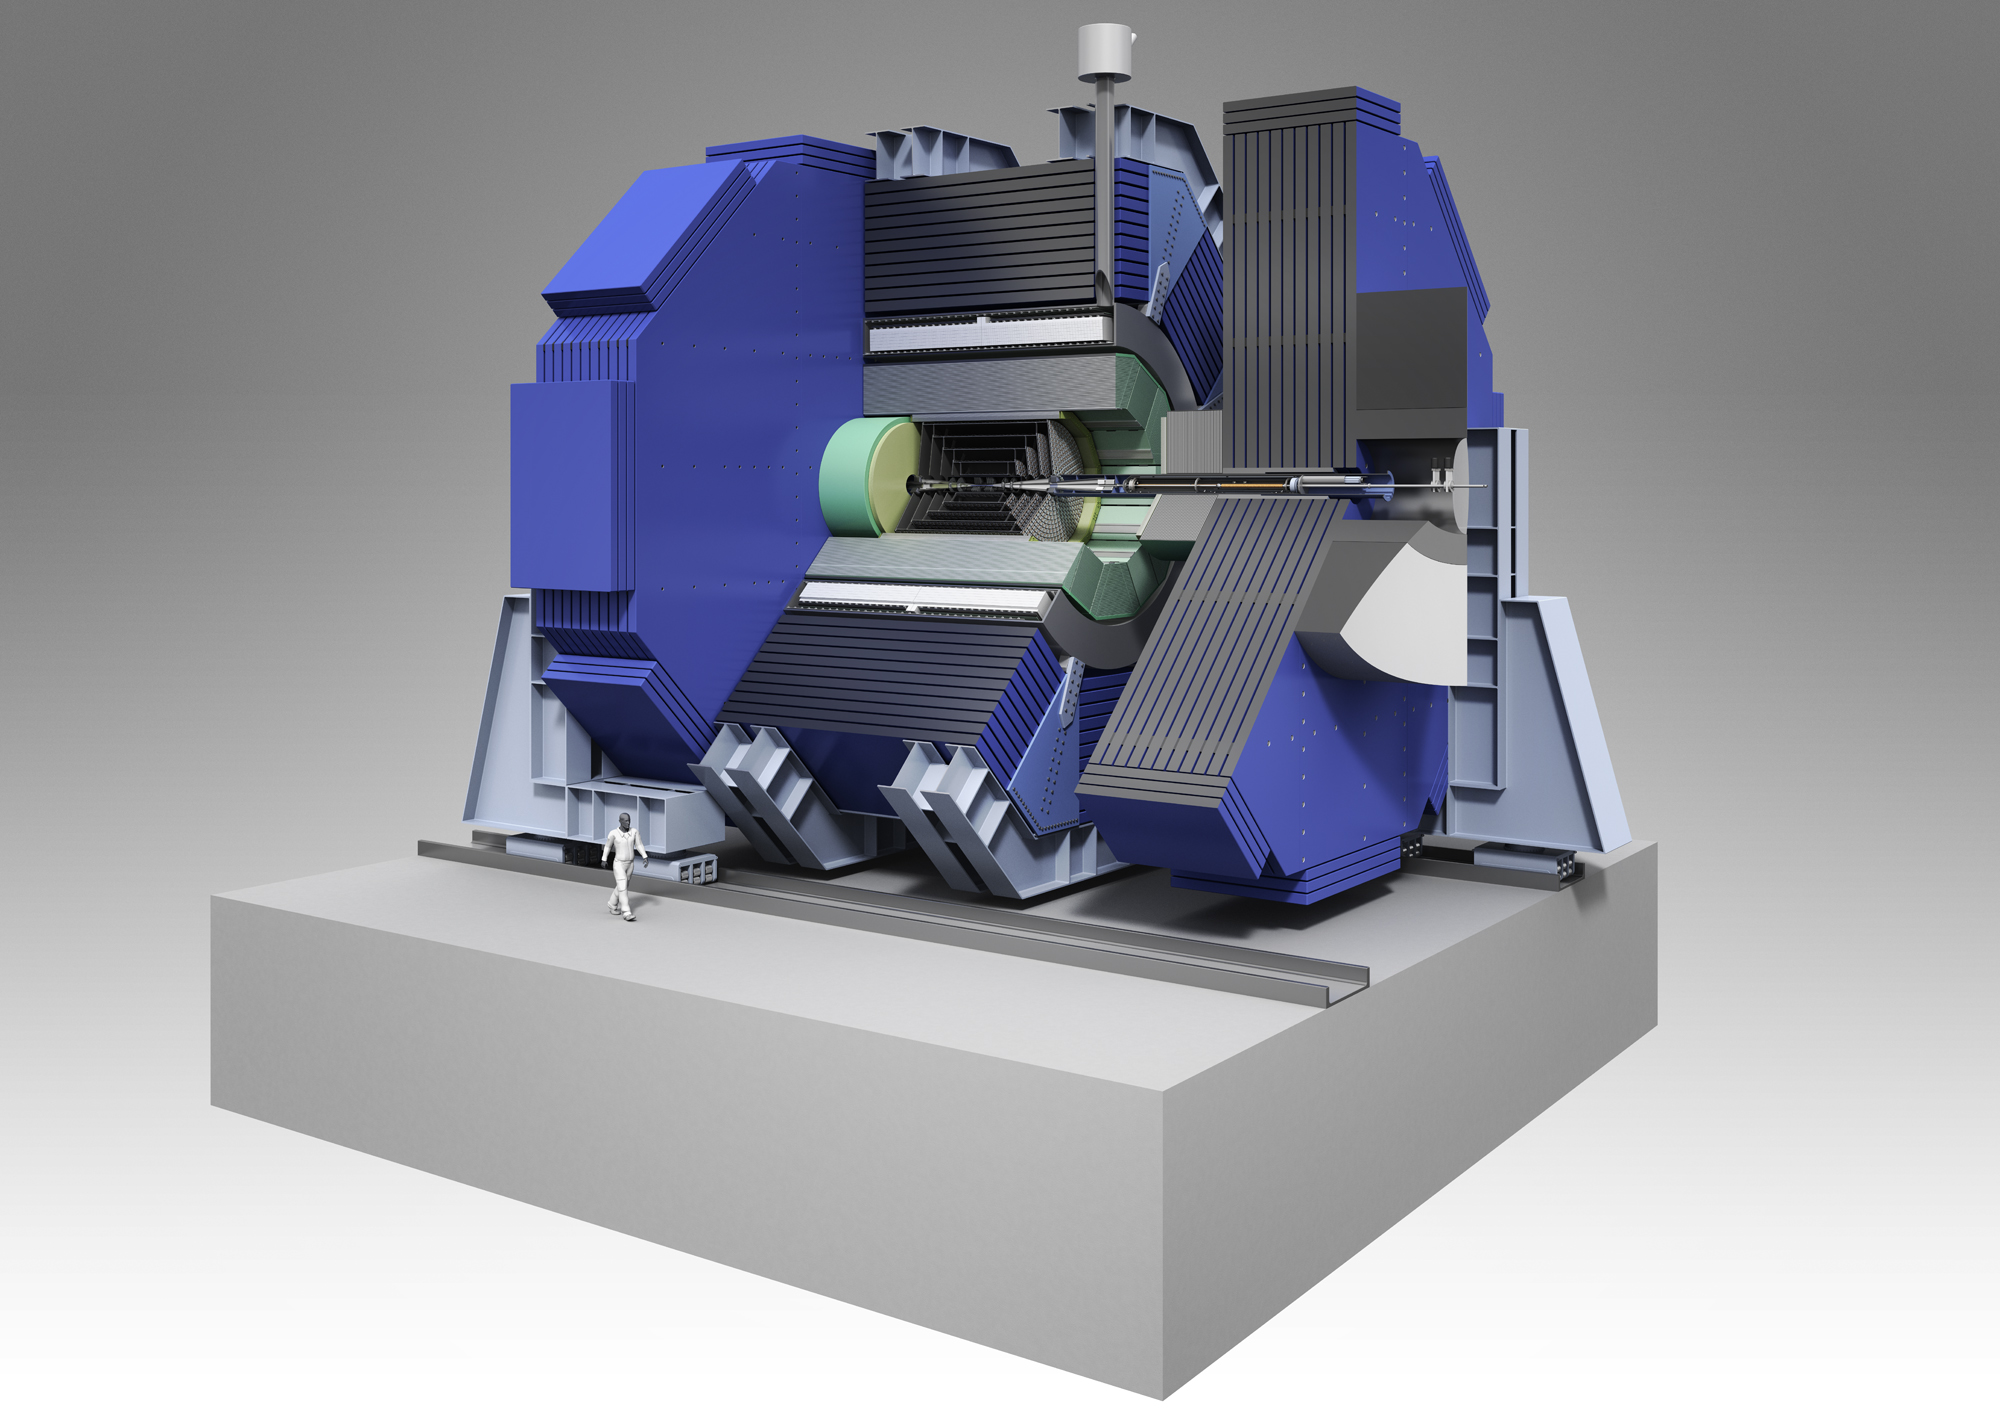
\includegraphics[width=0.45\textwidth]{figures/SiDmodel.jpg}\\
$\rightarrow$ SiD is a compact detector, designed for Particle Flow.
}
\end{center}
\end{column}
\begin{column}{0.5\textwidth}
\begin{center}
\visible<2->{\alert{ILD - International Large Detector}
\begin{itemize}
\item Height: $\sim$\SI{16}{\metre}, length:  $\sim$\SI{14}{\metre}
\item Weight: $\sim$\SI{14000}{\tonne}
\item Supercond. solenoid field: \SI{3.5}{\tesla}
\item TPC
\end{itemize}
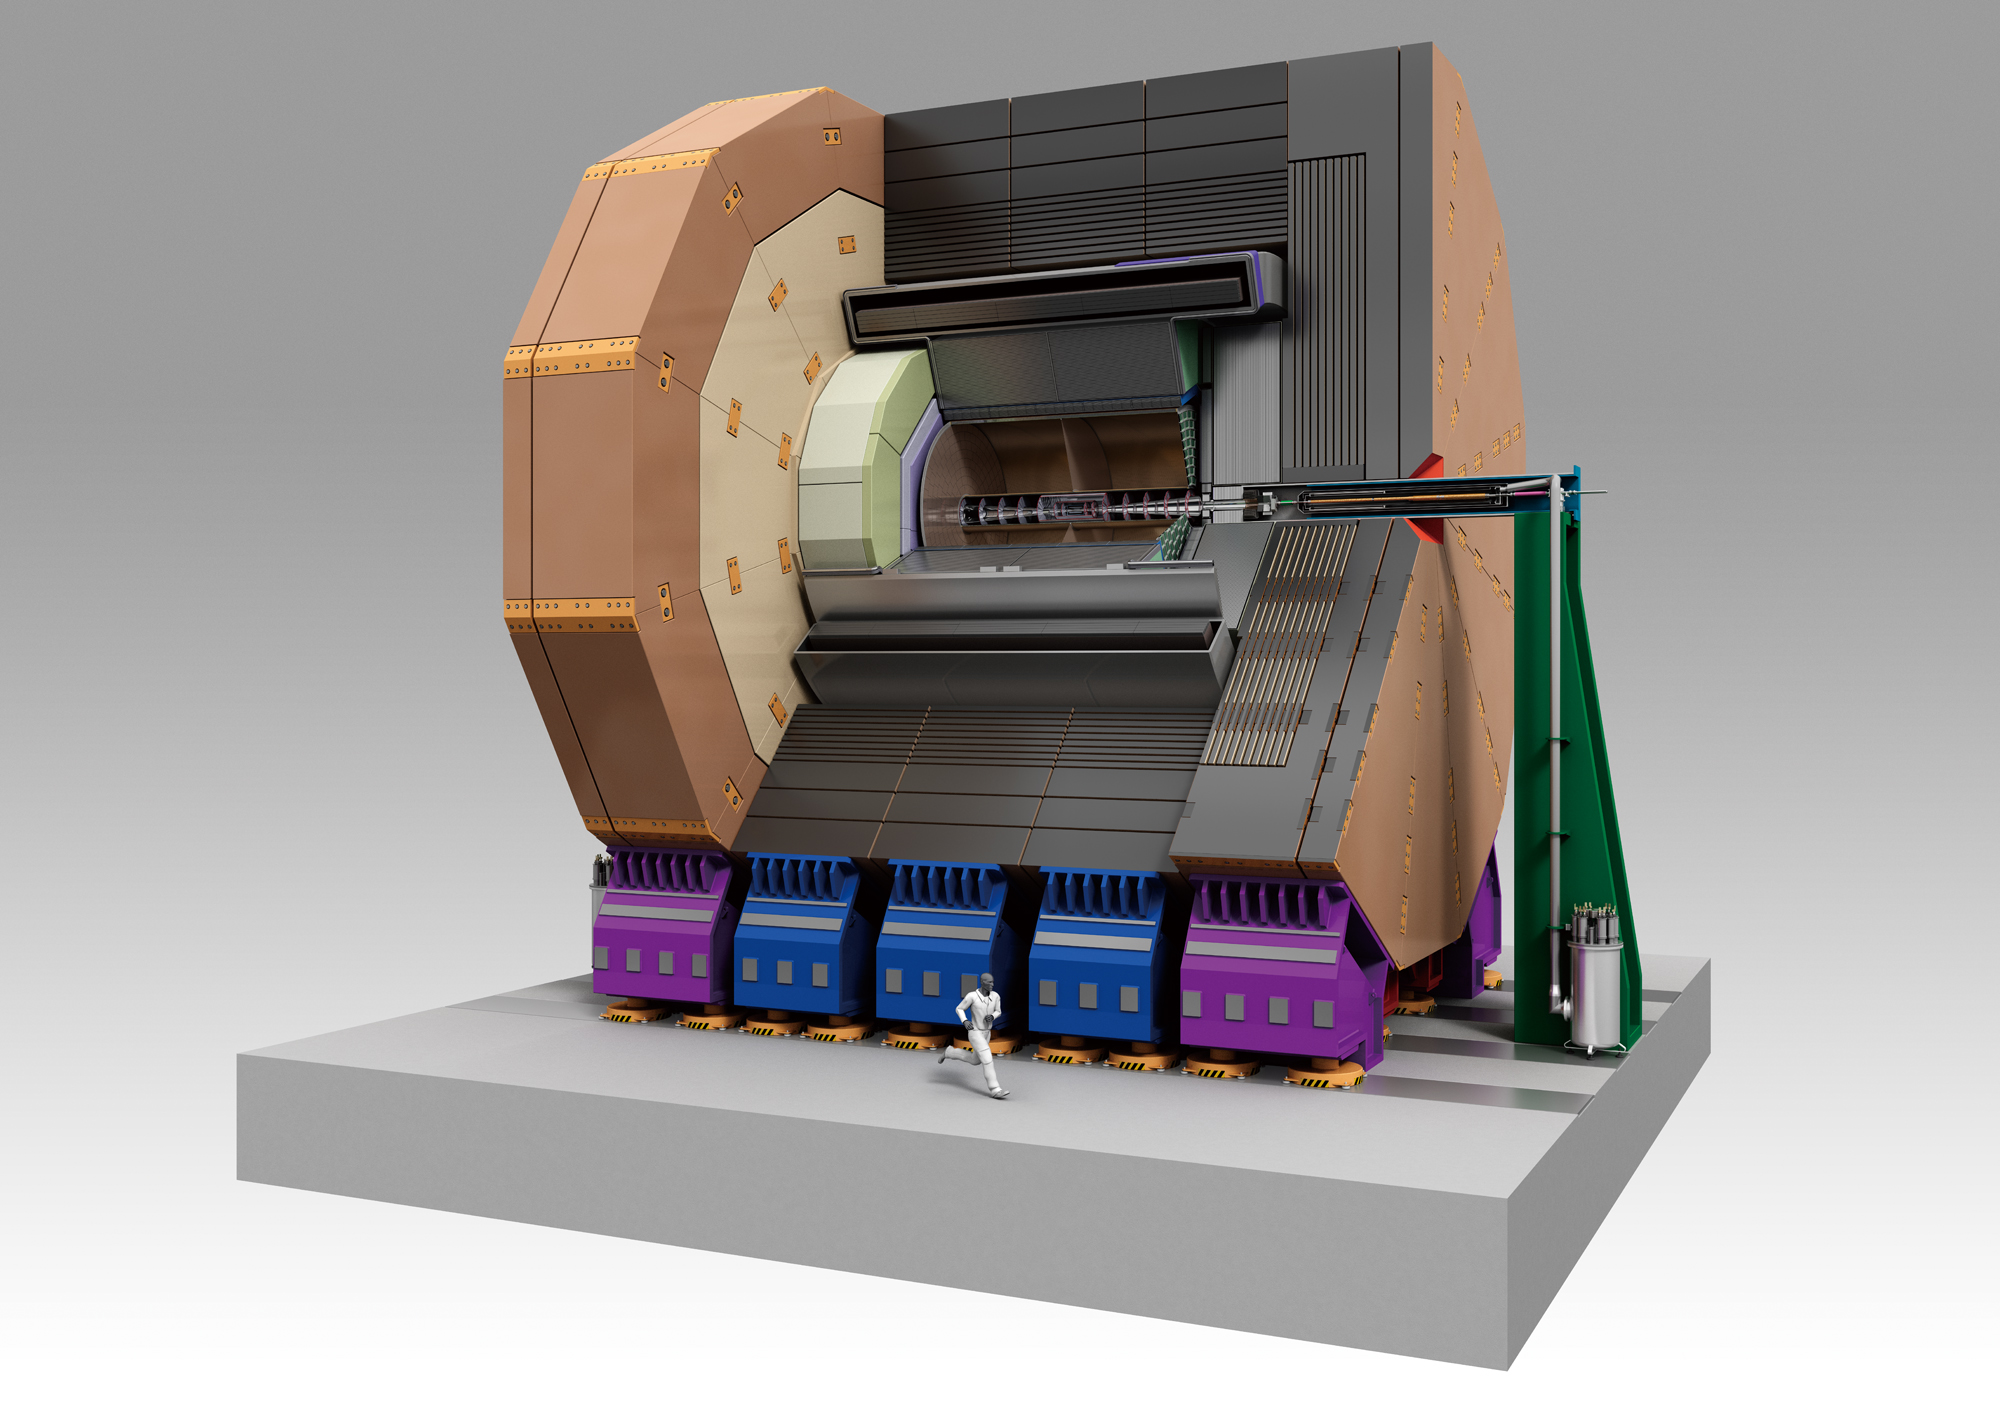
\includegraphics[width=0.45\textwidth]{figures/ILDmodel.jpg}\\
\textcolor{white}{line filler line filler line filler line filler line filler}
}
\end{center}
\end{column}
\end{columns}

\end{frame}

\begin{frame}{SiD detector}
\sidlogo
\begin{figure}[T]
\centering
\begin{subfigure}[b]{0.49\textwidth}
\centering
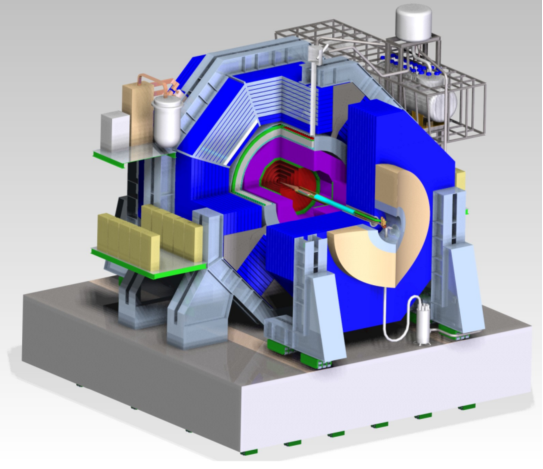
\includegraphics[height=0.65\textheight]{figures/SiD_detector_model.pdf}
\end{subfigure}
\begin{subfigure}[b]{0.49\textwidth}
\centering
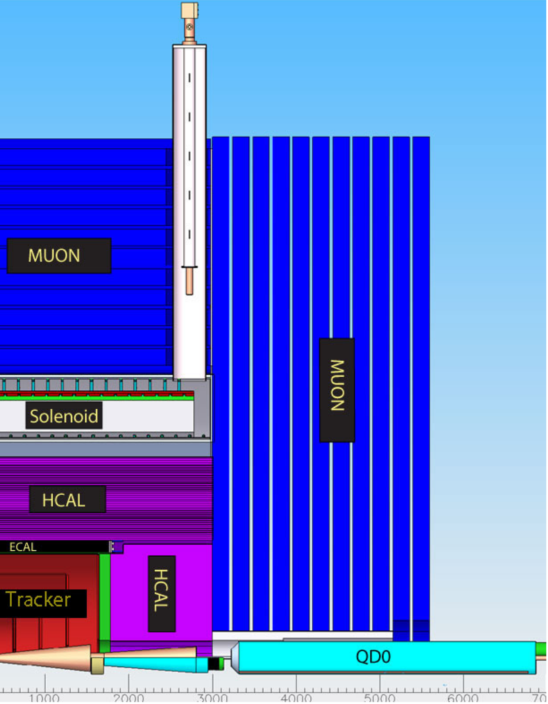
\includegraphics[height=0.65\textheight]{figures/SiD_detector_model_Ausschnitt.pdf}
\end{subfigure}
\caption{\small SiD detector model: Vertex detector (red), ECAL (green), HCAL (pink), Muon system (blue)}
\end{figure}
\end{frame}
%--------------------------------------------------------------

\section{Background simulation and Final-Focus optimization}

\subsection{Background sources at the ILC}
\begin{frame}{Background simulation \& Final-Focus optimization}
\ilclogo
\begin{block}{}
\centering The ILC will be a \textcolor{Periwinkle}{high luminosity} particle accelerator \\with \textcolor{JungleGreen}{extraordinary precision}.
\end{block}
\vspace*{1cm}
\textcolor{JungleGreen}{The high precision depends on the cleanliness}, \textcolor{Periwinkle}{the high luminosity on the capability to focus the beam to nanometer size}.\\
\vspace*{0.5cm}
In order to minimize the effect of the background on the detectors and the measurements, the different \textbf{background sources need to be modeled in great detail}, also with respect to a possible optimization of the Final-Focus layout.
\end{frame}

\begin{frame}{Background sources}
\ilclogo
The main sources of background:
\begin{columns}
 \begin{column}{0.6\textwidth}
  \begin{itemize}
    \item Beam-beam interactions:
    \begin{itemize}
      \item \textbf{Pair background}
      \item Bhabha scattering
      \item \textgamma \textgamma $\rightarrow$ hadrons
    \end{itemize}
    \vspace*{0.5cm}
    \item Machine background:
    \begin{itemize}
      \item \textbf{Muons from the Beam Delivery System}
      \item Neutrons from the Beam Dumps
      \item Background from the Final-Focus system (beam halo collimators)
    \end{itemize}
  \end{itemize}
 \end{column}
 \begin{column}{0.45\textwidth}
 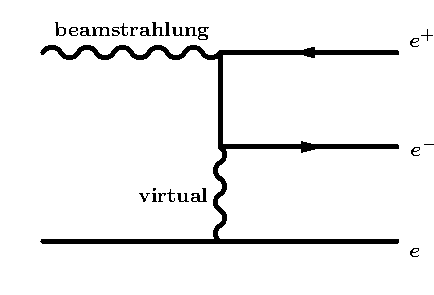
\includegraphics[width=0.33\textwidth]{figures/Bethe-Heitler.pdf}
 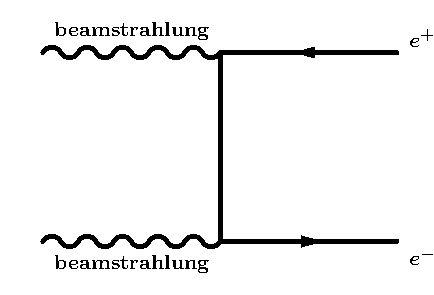
\includegraphics[width=0.33\textwidth]{figures/Breit-Wheeler.pdf}
 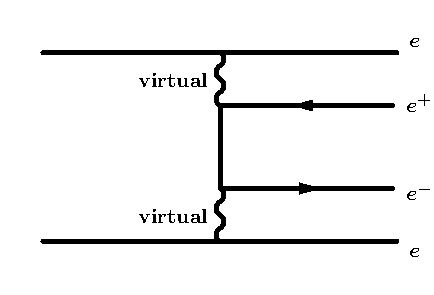
\includegraphics[width=0.33\textwidth]{figures/Landau-Lifshitz.pdf}\\
 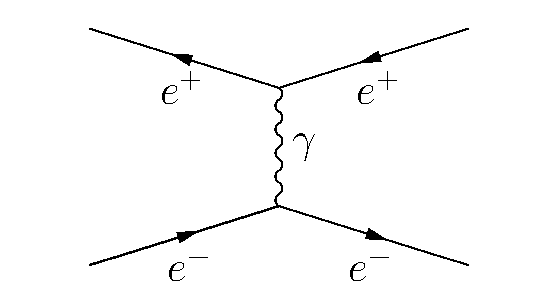
\includegraphics[height=0.15\textheight]{figures/bhabha_scattering.pdf} 
 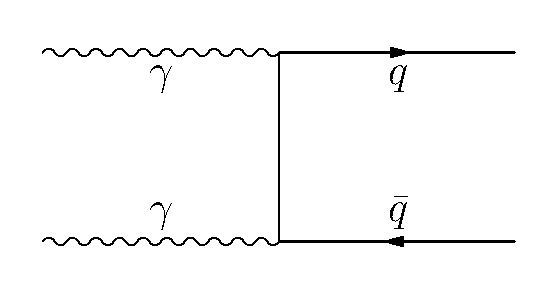
\includegraphics[height=0.15\textheight]{figures/gammagamma_hadrons.pdf}\\
 \vspace*{0.5cm}
 \includegraphics[width=0.8\textwidth]{figures/wall_shielding.png}
 \end{column}
\end{columns}
\end{frame}


\subsection{Pair background}

\begin{frame}{Pair background - Helix Envelopes for the ILC500}
\sidlogo
Per bunch, there are about \num{200000} \positron \electron background particles from beam-beam interactions.\\
Due to their momentum distributions, the particles form \textbf{helix tracks} in the solenoid field, resulting in envelopes of a characteristic shape.\\
\vspace*{0.1cm}
   \includegraphics[height=0.47\textheight]{figures/PairHelixes_500GeV_5T_10bunches_xz.png}\hspace*{0.1cm}
   \includegraphics[height=0.47\textheight]{figures/HelixEnvelopes_Helix_tracks_xz_Helix_10bunches_500GeV_5T.png}\\
The envelopes show that at any given point the beam pipe is 4mm away from 99.9\% of all pair particle tracks.\\
\textbf{$\Rightarrow$ Reducing the beam pipe \& vertex detector radius} by $\sim$2mm.
\end{frame}
%\begin{frame}{Pair background envelopes - 350GeV}
%   \includegraphics[width=0.51\textwidth]{figures/PairHelixes_350GeV_5T.png}\hspace*{0.1cm}
%   \includegraphics[width=0.51\textwidth]{figures/PairEnvelopes_350GeV_5T.png}
%\end{frame}
%\begin{frame}{Pair background envelopes - 250GeV}
%   \includegraphics[width=0.51\textwidth]{figures/PairHelixes_250GeV_5T.png}\hspace*{0.1cm}
%   \includegraphics[width=0.51\textwidth]{figures/PairEnvelopes_250GeV_5T.png}
%\end{frame}

\subsection{Muons from the BDS}
\begin{frame}
 \vspace*{3cm}
 \begin{center}
  \LARGE Muons from the Beam Delivery System (BDS)
 \end{center}
 \vspace*{3cm}
\begin{flushright}
 \small In collaboration with\\Jonas Glombitza (RWTH Aachen)
\end{flushright}

\end{frame}

  \begin{frame}{The Beam Delivery System}
\begin{center}
  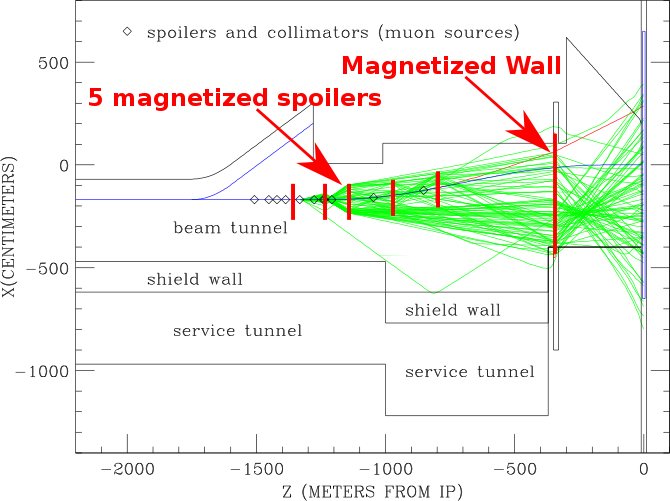
\includegraphics[width=0.7\textwidth]{figures/BDS_Tunnel_Spoilers+Wall.png}
\end{center}
Muons are created along the BDS, when the beam halo interacts with the beam line material.
\end{frame}

\begin{frame}{The Muon Spoilers}
\begin{columns}
 \begin{column}{0.4\textwidth}
 The two suggested shielding scenarios:
  \begin{itemize}
   \item \textbf{5 Spoilers}
   \begin{itemize}
    \item 70cm radius, 5m long
    \item magnetized iron
    \item at 5 locations along the BDS
   \end{itemize}
   \item \textbf{5 Spoilers + Wall}
    \begin{itemize}
    \item 4m x 5m, 5m long
    \item magnetized iron
    \item close to the interaction region
   \end{itemize}
  \end{itemize}

 \end{column}
 \begin{column}{0.6\textwidth}
  \fbox{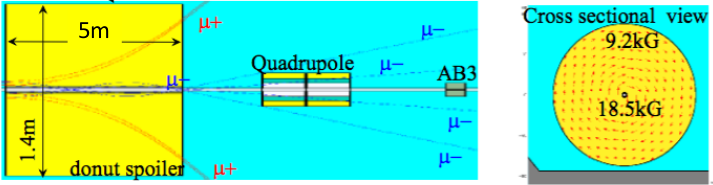
\includegraphics[width=\textwidth]{figures/Spoiler.png}}\\\vspace*{0.3cm}
  \fbox{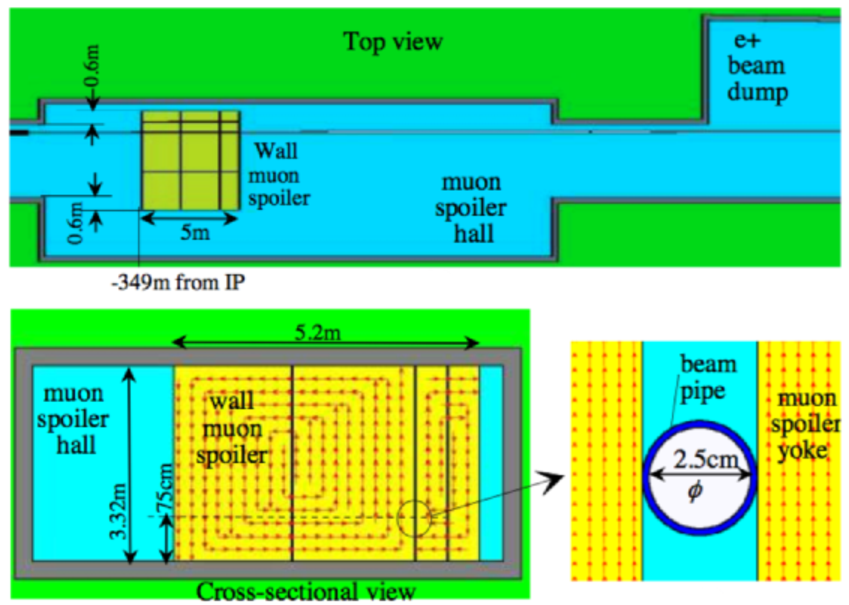
\includegraphics[width=\textwidth]{figures/Muon_wall.pdf}}
 \end{column}
\end{columns} 
\end{frame}

\begin{frame}{WIRED4 event display - 5 Spoilers + Wall}
\sidlogo
1 train's worth of muons ($\sim$ 515 muons) \textbf{from the positron line only}:
\begin{center}
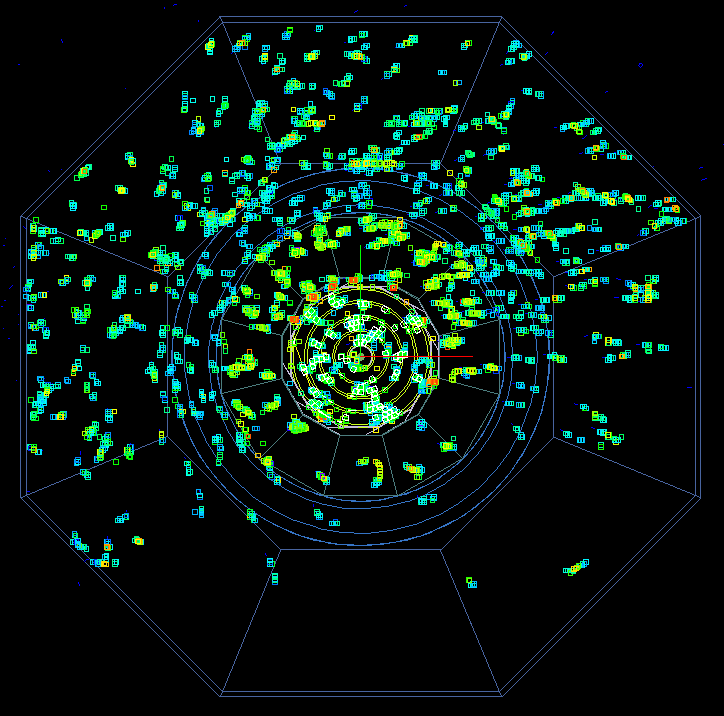
\includegraphics[height=0.6\textheight]{figures/muons_positron_5spoilers_wall_515_xyview_croped.png}
{\tiny xy-view}
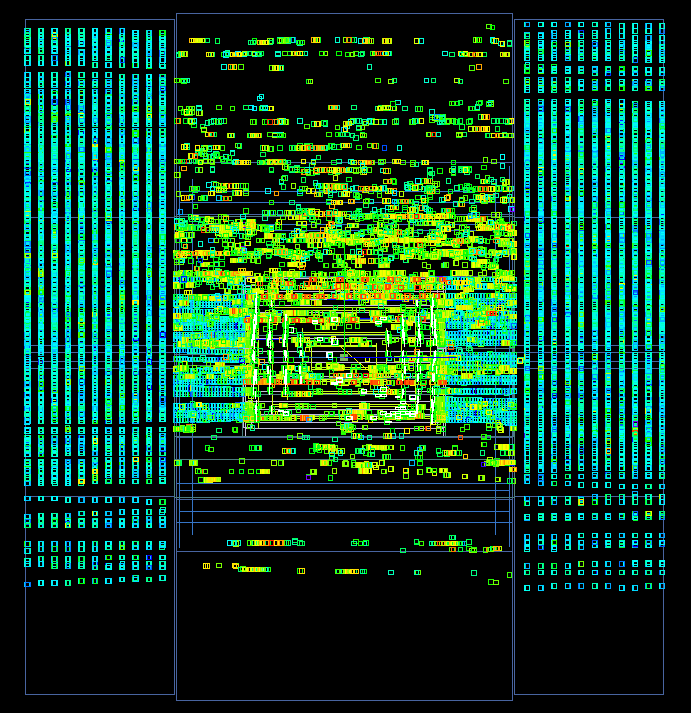
\includegraphics[height=0.6\textheight]{figures/muons_positron_5spoilers_wall_515_zyview_croped.png}
{\tiny zy-view}
\end{center}
Together with the muons from the e\textsuperscript{-} line, there will be \textbf{$\sim$ 900 muons per train in the '5 Spoilers + Wall' scenario}.
\end{frame}
\begin{frame}{WIRED4 event display - 5 Spoilers}
\sidlogo
1 train's worth of muons ($\sim$ 2961 muons) \textbf{from the positron line only}:
\begin{center}
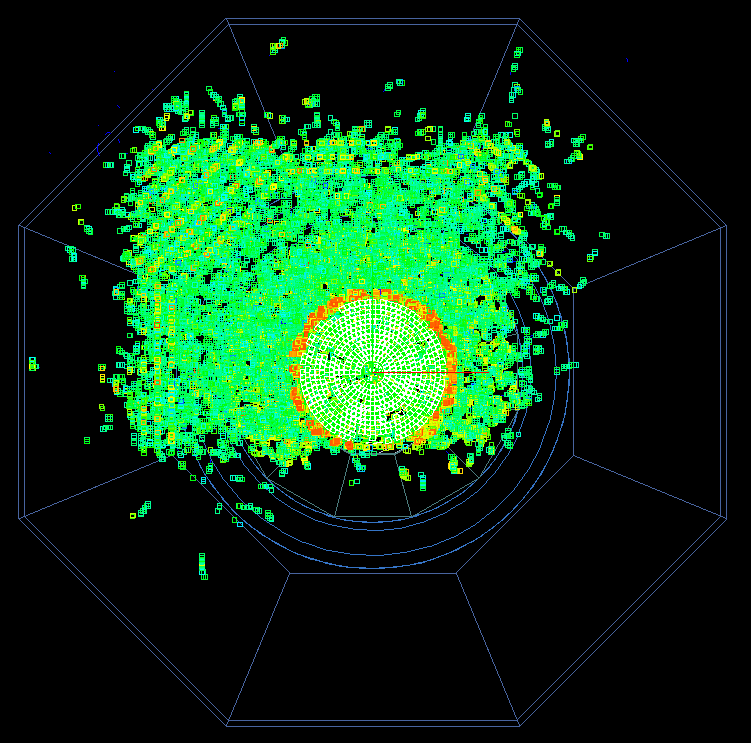
\includegraphics[height=0.6\textheight]{figures/muons_positron_5spoilers_2961_xyview_croped.png}
{\tiny xy-view}
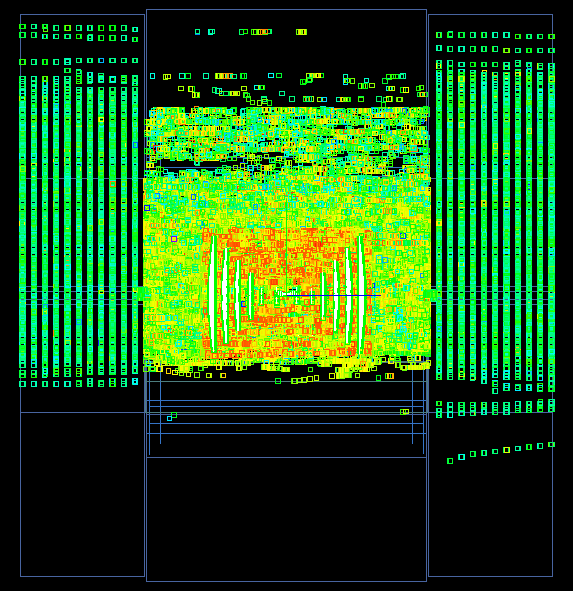
\includegraphics[height=0.6\textheight]{figures/muons_positron_5spoilers_2961_zyview_croped.png}
{\tiny zy-view}
\end{center}
Together with the muons from the e\textsuperscript{-} line, there will be \textbf{$\sim$ 5600 muons per train in the '5 Spoilers' scenario}.\\
The spatial distribution is due to the tunnel shape and its shielding effects.
\end{frame}


 
\begin{frame}{The Muon Occupancy in SiD ECAL endcaps}
\sidlogo
\begin{center}
  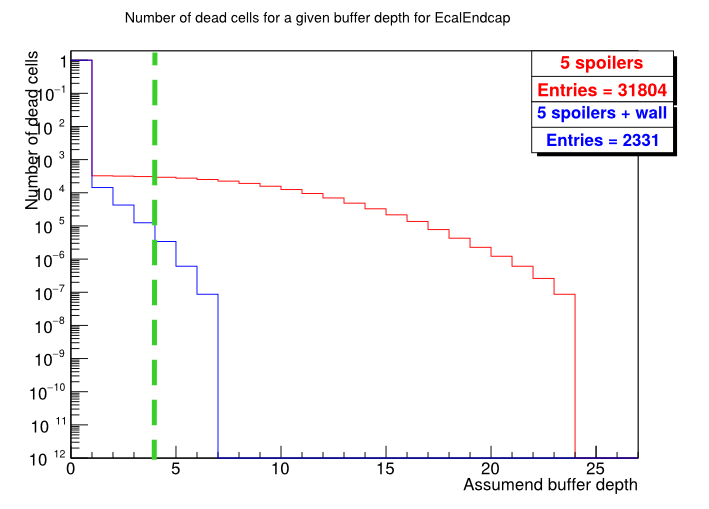
\includegraphics[width=0.61\textwidth]{figures/EcalEndcap_DeadCells.png}
\end{center}
{\small A readout cell is ``dead'' when all buffers of the sensor are already filled. No more hits can be stored.}\\
The current SiD electronics design has a \textcolor{Green}{buffer depth of 4}, i.e. \textcolor{Blue}{10\textsuperscript{-6}} - \textcolor{Red}{10\textsuperscript{-4}} of all hits are dead in the ECAL endcaps.
\end{frame}

\begin{frame}
 With the shown results from the muon occupancy analysis, the \textbf{SiD group prefers to keep the magnetized wall} in order to keep the occupancy in the SiD detector as low as possible.\\
 \vspace*{0.5cm}
 \begin{columns}
  \begin{column}{0.4\textwidth}
    This will also \textbf{allow access to the detector parking garage}, since the wall represents a \textbf{tertiary containment device} against not only muons but also photons and neutrons from the machine background.
  \end{column}
  \begin{column}{0.6\textwidth}
    \includegraphics[width=\textwidth]{figures/wall_shielding.png}
  \end{column}
 \end{columns}
\end{frame}

\section{Summary and Conclusion}
\begin{frame}
\textit{Suggestions for design improvements for the ILC:}
 \begin{itemize} 
  \item Looked at the \textbf{pair helix envelopes} for 500 \textcolor{Gray}{(350 and 250GeV)} ILC staging scenarios \textcolor{Green}{$\rightarrow$ suggested \textbf{reducing the radius of beam pipe and vertex detector}}
  \item Studied two different \textbf{muon shielding possibilies} and the muon occupancy in SiD \textcolor{Green}{$\rightarrow$ \textbf{Spoilers + Wall} is \textbf{prefered} shielding option}
 \end{itemize}
\textit{Further performance studies and suggestions for design improvements have been done or are ongoing:}
 \begin{itemize}
  \item Studied the \textbf{timing and origin of pair background and backscattering particles} \textcolor{Green}{$\rightarrow$ possible reduction of background with \textbf{time gates}}
  \item \textbf{Simulating the Beam Dump with FLUKA} in collaboration with Benno List (DESY)
  \item Study possible \textbf{improvement in physics event reconstruction when reducing the beam pipe and vertex detector radius}, whilst looking at the increase in background level at such radii
 \end{itemize}
\end{frame}


\section*{The end}
{
\usebackgroundtemplate{
 \tikz\node[opacity=0.1]{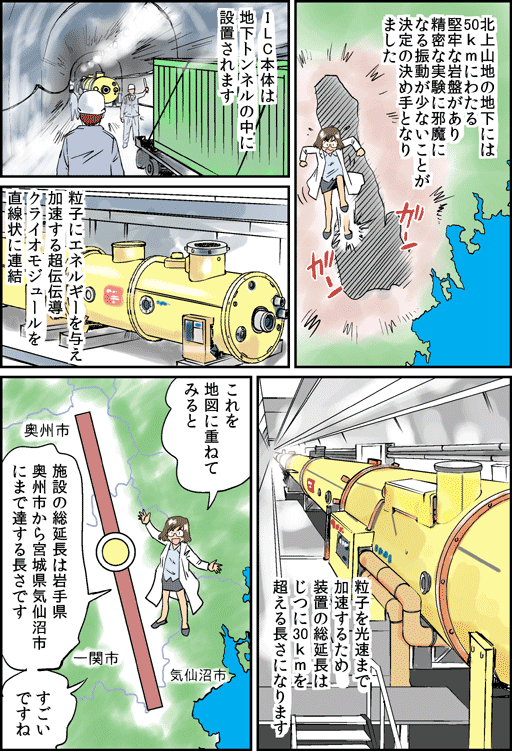
\includegraphics[width=\paperwidth,resolution=200]{figures/ilc-Comic.png}};
 % \tikz\node[opacity=0.2]{\centering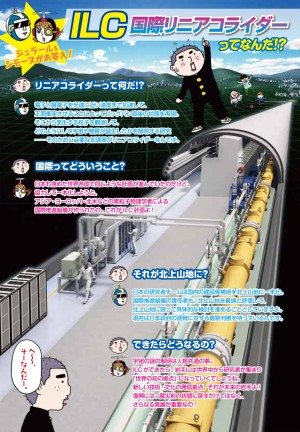
\includegraphics[height=\paperheight]{figures/Iwatecomics.jpg}};
 }
\begin{frame}
\ilclogo
\begin{center}
If you are interested in SiD and keen on working for the ILC, \\
if you like working in a very international environment, \\
or if you love Japan,\\
there are lots of possible Master's and Ph.D topics.\\
\vspace*{1cm}
\textcolor{RubineRed}{
	\LARGE Thanks!\\
	\begin{CJK}{UTF8}{min}
	どうもありがとうございます。
	\end{CJK}
}
\end{center}
\end{frame}
}

\section*{References}
\begin{thebibliography}{9}
\begin{frame}{References}
\bibitem{TDR} T. Behnke, et al.
\emph{The International Linear Collider - Technical Design Report}, 2013.
\bibitem{LHC TDR} \emph{LHC - Design Report}, \url{http://ab-div.web.cern.ch/ab-div/Publications/LHC-DesignReport.html}
\bibitem{IP beam parameters} ATLAS-CONF-2010-027. \emph{Characterization of Interaction-Point Beam Parameters Using the pp Event-Vertex Distribution Reconstructed in the ATLAS Detector at the LHC}, 2010. \url{http://cds.cern.ch/record/1277659/files/ATLAS-CONF-2010-027.pdf}
\end{frame}
\end{thebibliography}

%--------------------------------------------------------------------------------
\appendix

\begin{frame}
\begin{center}
\LARGE Additional Material
\end{center}
  \tableofcontents
\end{frame}

\section{ILC}


%------Definition for column color in table
\definecolor{Gray}{gray}{0.9}
\newcolumntype{g}{>{\columncolor{Gray}}r}
%-----------------------------------------
\subsection{The beam parameters}
\begin{frame}{The beam parameters of the ILC}
\ilclogo

\begin{table}[]
\centering
\begin{tabularx}{\textwidth}{ll|rrrg}
\hline
& & \multicolumn{1}{>{\centering}p{1.5cm}}{\textbf{Baseline 500}} & \multicolumn{1}{>{\centering}p{1.5cm}}{\textbf{Lumi Upgrade}} & \multicolumn{1}{>{\centering}p{1.5cm}}{\textbf{TeV Upgrade}} & {\centering\textbf{LHC 25ns}} \\ 
\hline
\cline{1-6}
\hline
E$_{CM}$  &[\si{\GeV}] & 500  & 500  & \num{1000} & \num{14000}\\
n$_b$ & & \num{1312} & \num{2625} & \num{2450} &  \num{2808} \\
$\Delta t_b$ &[\si{\nano\second}] & 554  & 366   & 366 & 25 \\
N & & \num{2.0e10}  & \num{2.0e10}  & \num{1.74e10}  & \num{11.5e10}\\
q$_b$ &[\si{\nano\coulomb}] & 3.2  & 3.2  &  2.7 & 18.4 \\
$\sigma_x^*$ &[\si{\nano\metre}] & 474  & 474  &  481 & \num{16700}\\
$\sigma_y^*$ &[\si{\nano\metre}] & 5.9 &  5.9  &  2.8 & \num{16700}\\
$\sigma_z$ &[\si{\milli\metre}] & 0.3  &  0.3  &  0.25 & 0.755\\
L &[\si{\per\centi\metre\squared\per\second}] & \num{1.8e34} & \num{3.6e34} & \num{3.6e34} & \num{1.0e34}\\
\hline
\end{tabularx}
\end{table}
\end{frame}


\subsection{ILC baseline parameters}
\begin{frame}{ILC baseline parameters}
\ilclogo
\centering
	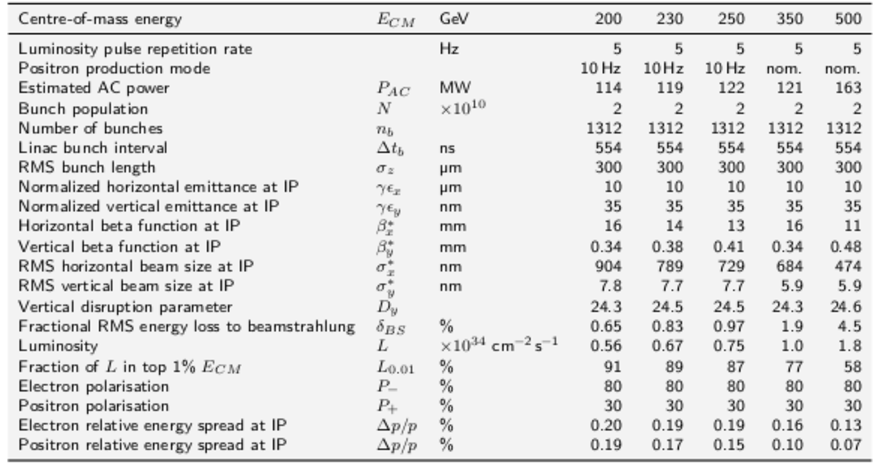
\includegraphics[width=\textwidth]{figures/ILCTDR-VOLUME_3-PART_II_ILCparameters.pdf}
\end{frame}
\begin{frame}{ILC parameters for the different upgrade stages}
\ilclogo
\centering
	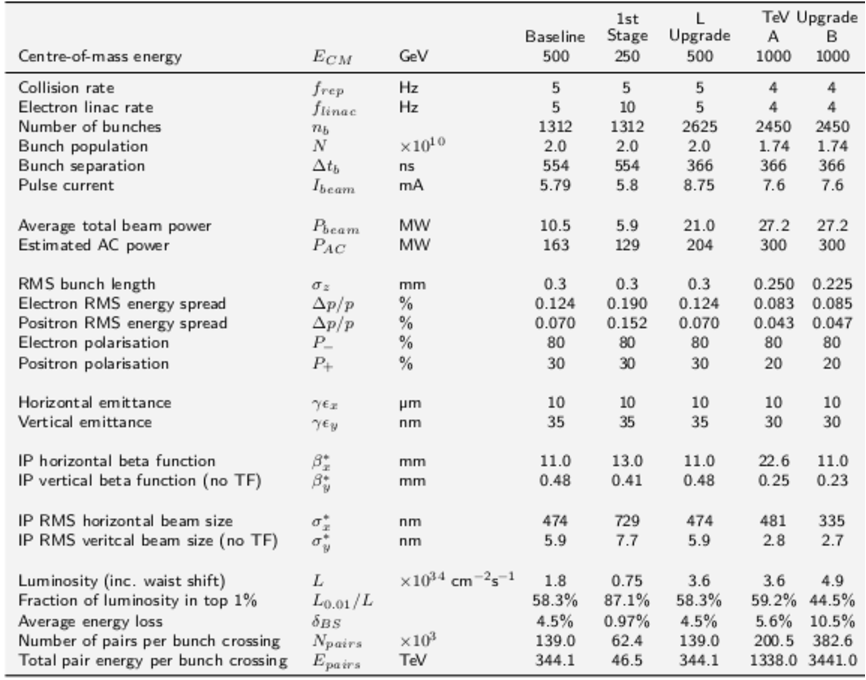
\includegraphics[width=0.8\textwidth]{figures/ILCTDR-VOLUME_3-PART_II_ILCparametersUpgrades.pdf}
\end{frame}

\begin{frame}{Why linear?}
\begin{columns}
 \begin{column}{0.6\textwidth}
  Basic limitations of lepton synchrotons:
\begin{itemize}
 \item \textcolor{Red}{Energy loss due to synchrotron radiation: $\sim$ E$^4$/R}
 \item \textcolor{Red}{Cost $\sim$ quadratically with energy}\\ \tiny{(B. Richter 
1980)}
\end{itemize}
\vspace*{1cm}
Therefore a linear collider:
\begin{itemize}
 \item \textcolor{ForestGreen}{Not limited by synchrotron radiation}
 \item \textcolor{ForestGreen}{Cost $\sim$ linear with energy}
\end{itemize}
 \end{column}
 \begin{column}{0.4\textwidth}
 \begin{block}{}
  \begin{center}
      \textcolor{CadetBlue}{P$_S=\frac{e^2c}{6\pi\epsilon_0}\frac{1}{(m_0c^2)^4}\frac{E^4}{R^2}$\\
  $\Delta$E$=\frac{e}{3\epsilon_0(m_0c^2)^4}\frac{E^4}{R}$}
   \end{center}
 \end{block}
 \end{column}
\end{columns}

\end{frame}

\subsection{SiD}
\begin{frame}{SiD detector}
\sidlogo
 I am in the SiD-Optimization group.\\
 Marcel Stanitzki is currently the SiD co-spokesperson.\\
 \vspace*{0.3cm}
 \visible<2->{
 \begin{columns}
  \begin{column}{0.7\textwidth}
    SiD has a very convincing design:
 \begin{itemize}
  \item compact and robust
  \item full silicon vertex detector and tracker
  \\Vertex detector:
  \begin{itemize}
   \item $<$\SI{5}{\micro\metre} resolution
   \item Momentum resolution $\sim$ 2-\SI{5e-5}{\per\giga\electronvolt}
   \item $\sim$ \SI{0.1}{\percent} X$_0$ per layer
  % \item Single bunch timing resolution
  % \item cos($\theta$)$\approx$0.984
  \end{itemize}

  \item highly granular calorimetry optimized for Particle Flow (ECAL: radation length = 26 X$_0$, \\EM energy resolution = 0.17/$\sqrt{E}\bigoplus$1\%)
 \end{itemize}
  \end{column}
  \begin{column}{0.3\textwidth}
    \begin{flushright}
  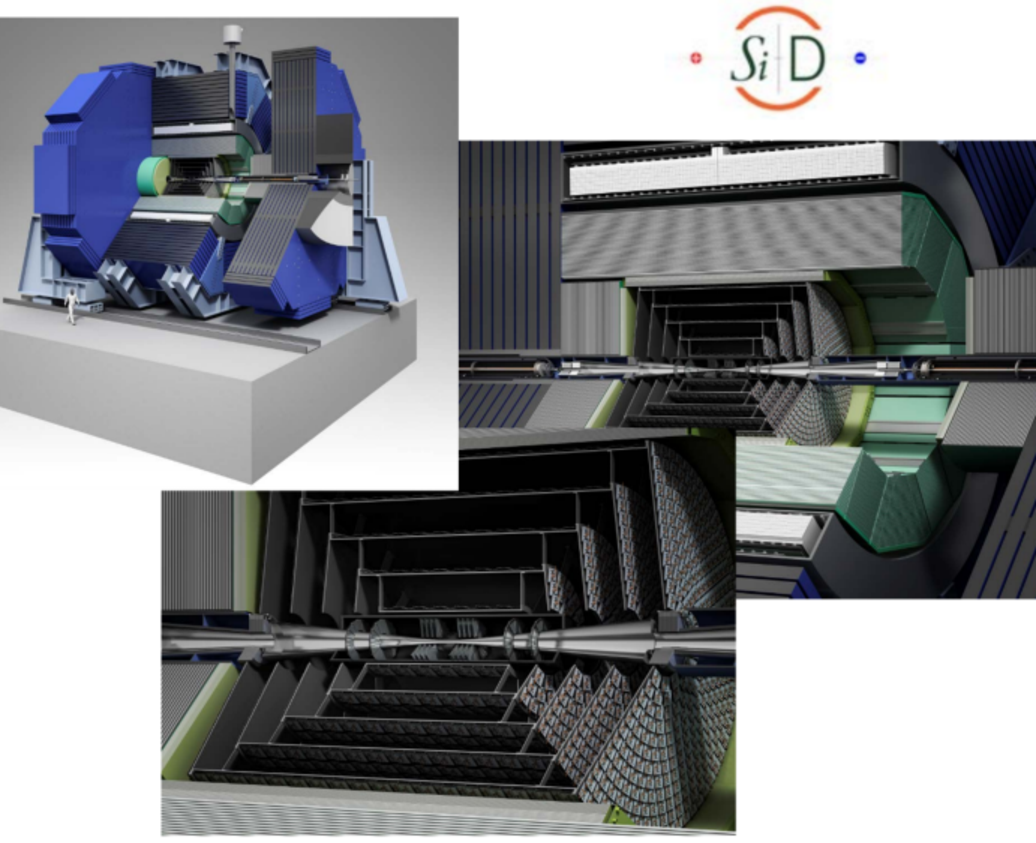
\includegraphics[height=0.4\textheight]{figures/SiDpics.pdf}
 \end{flushright}
  \end{column}
 \end{columns}
}
\end{frame}

\AtBeginSection[]
{
  \begin{frame}<beamer>
     \tableofcontents[
     currentsection,
     hideothersubsections]
  \end{frame}
}

\section{Pair background}

\subsection{Pair background helixes}
\begin{frame}{Explanation of helix track calculations}
 \begin{center}
  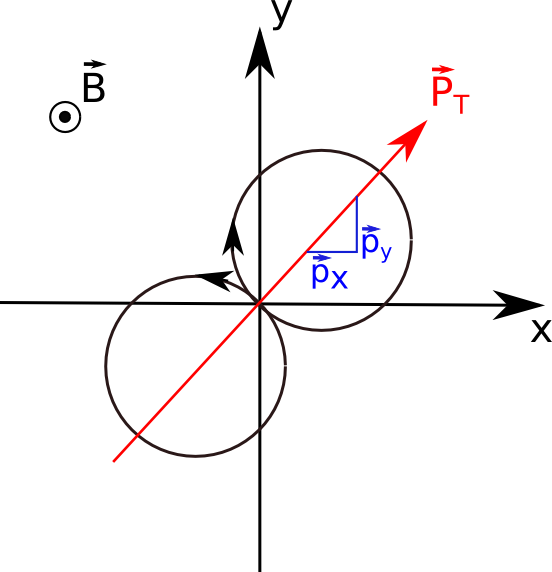
\includegraphics[width=0.65\textwidth]{figures/Helix_explanation.png}
\end{center}
\end{frame}
\begin{frame}{Pair background -  P\textsubscript{T}}
\sidlogo
Since their P\textsubscript{T} ranges between 0 and 2GeV, they form helix tracks in the solenoid field. The tracks extend to the inner detector layers, and leave up to several tens of hits.
\begin{center}
\includegraphics[width=0.7\textwidth]{figures/PT_hittime_primaries_SiVertexEndcapSiVertexBarrel.pdf}
\end{center}
\end{frame}


\section{Muons from the BDS}
\begin{frame}{The BDS}
\begin{center}
  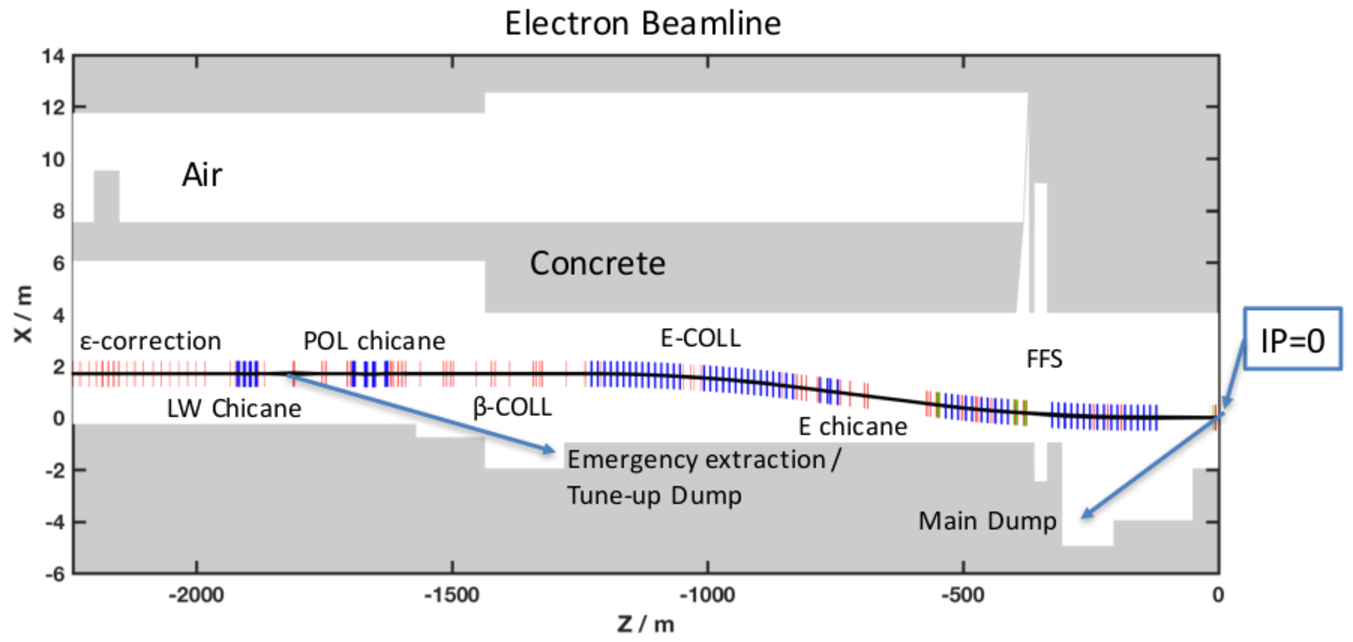
\includegraphics[width=0.9\textwidth]{figures/BDS_electron_tunnel.pdf}
  \end{center}
The Beam Delivery System (BDS) contains the Final Focus System, and therefore focusses the beam on its way to the Interaction Point (IP).
\end{frame}

\begin{frame}{The Muon Occupancy in SiD}
 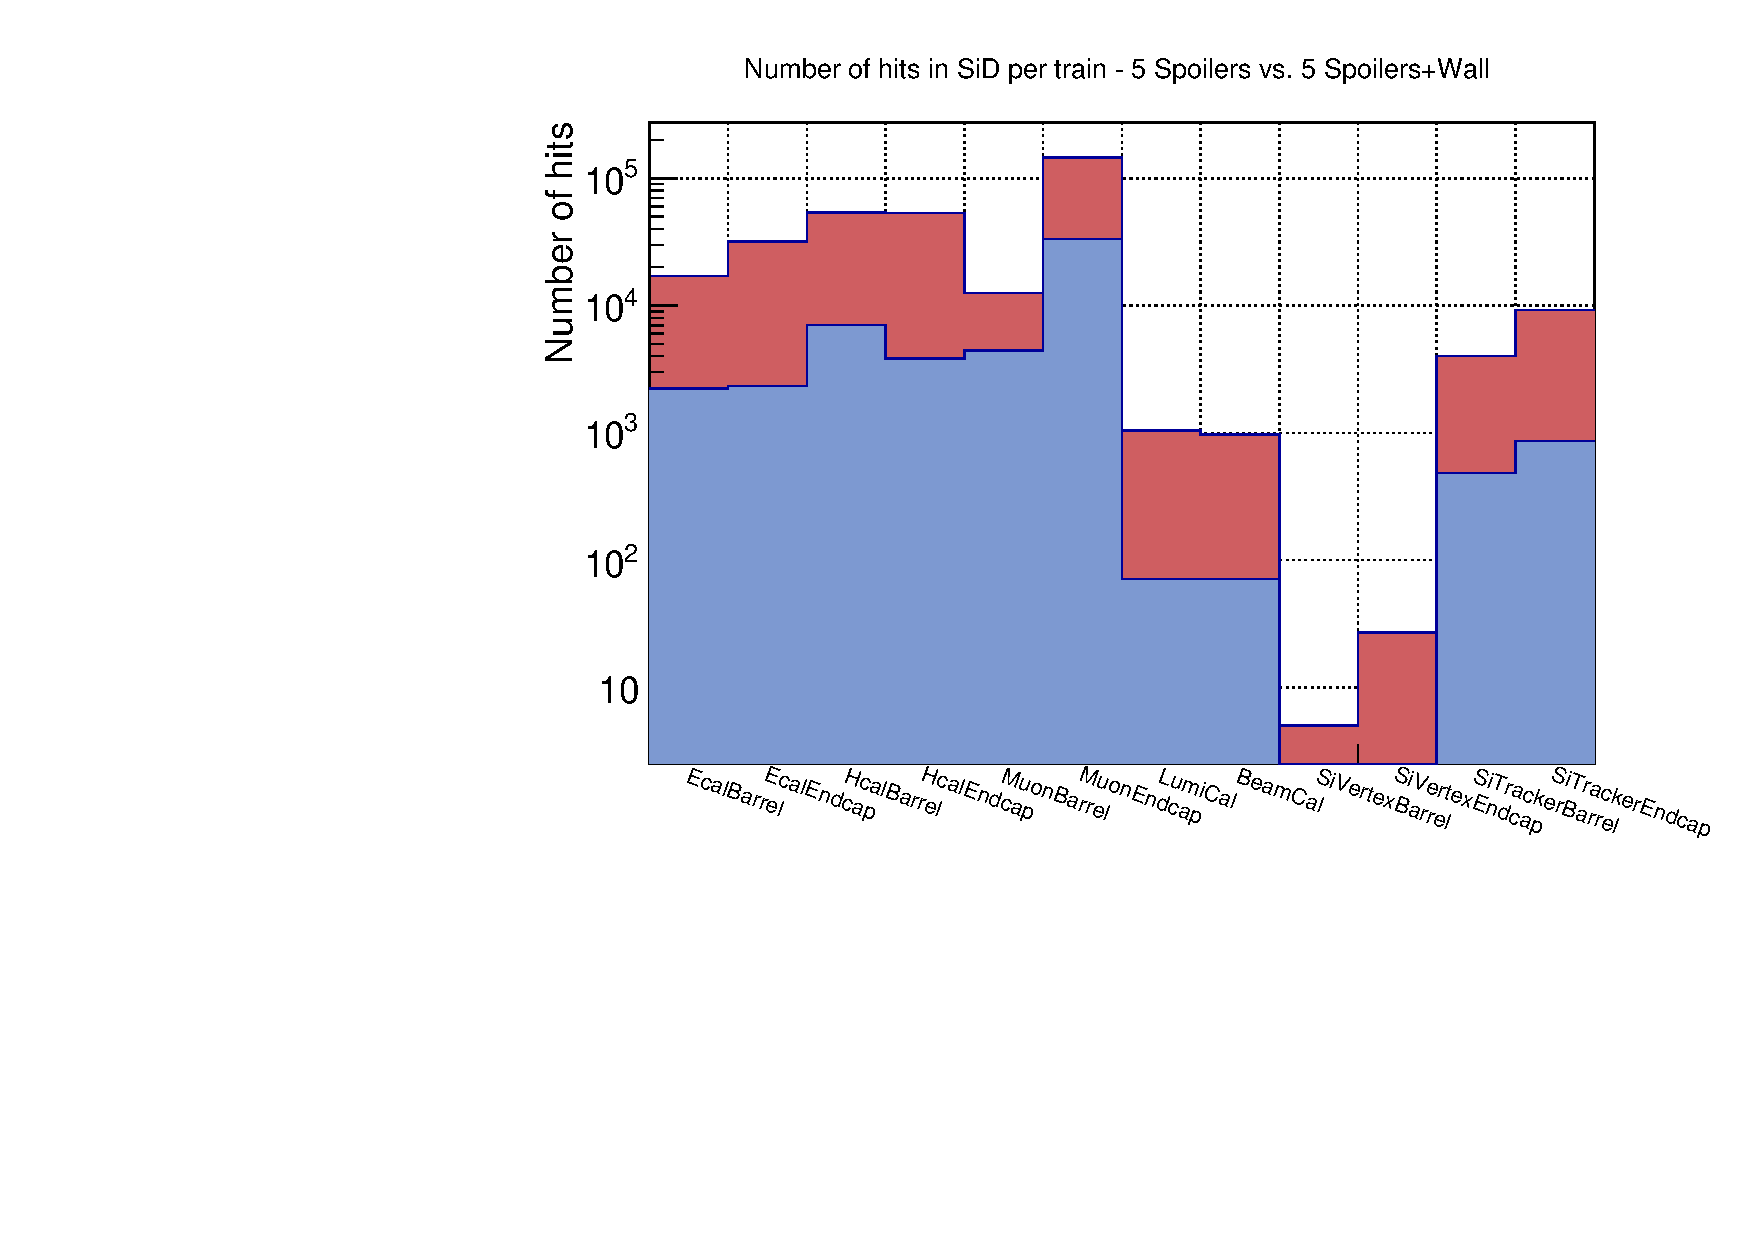
\includegraphics[width=0.6\textwidth]{figures/Hits_in_SiD_subdetectors_MuonSpoilerStudy.pdf}
  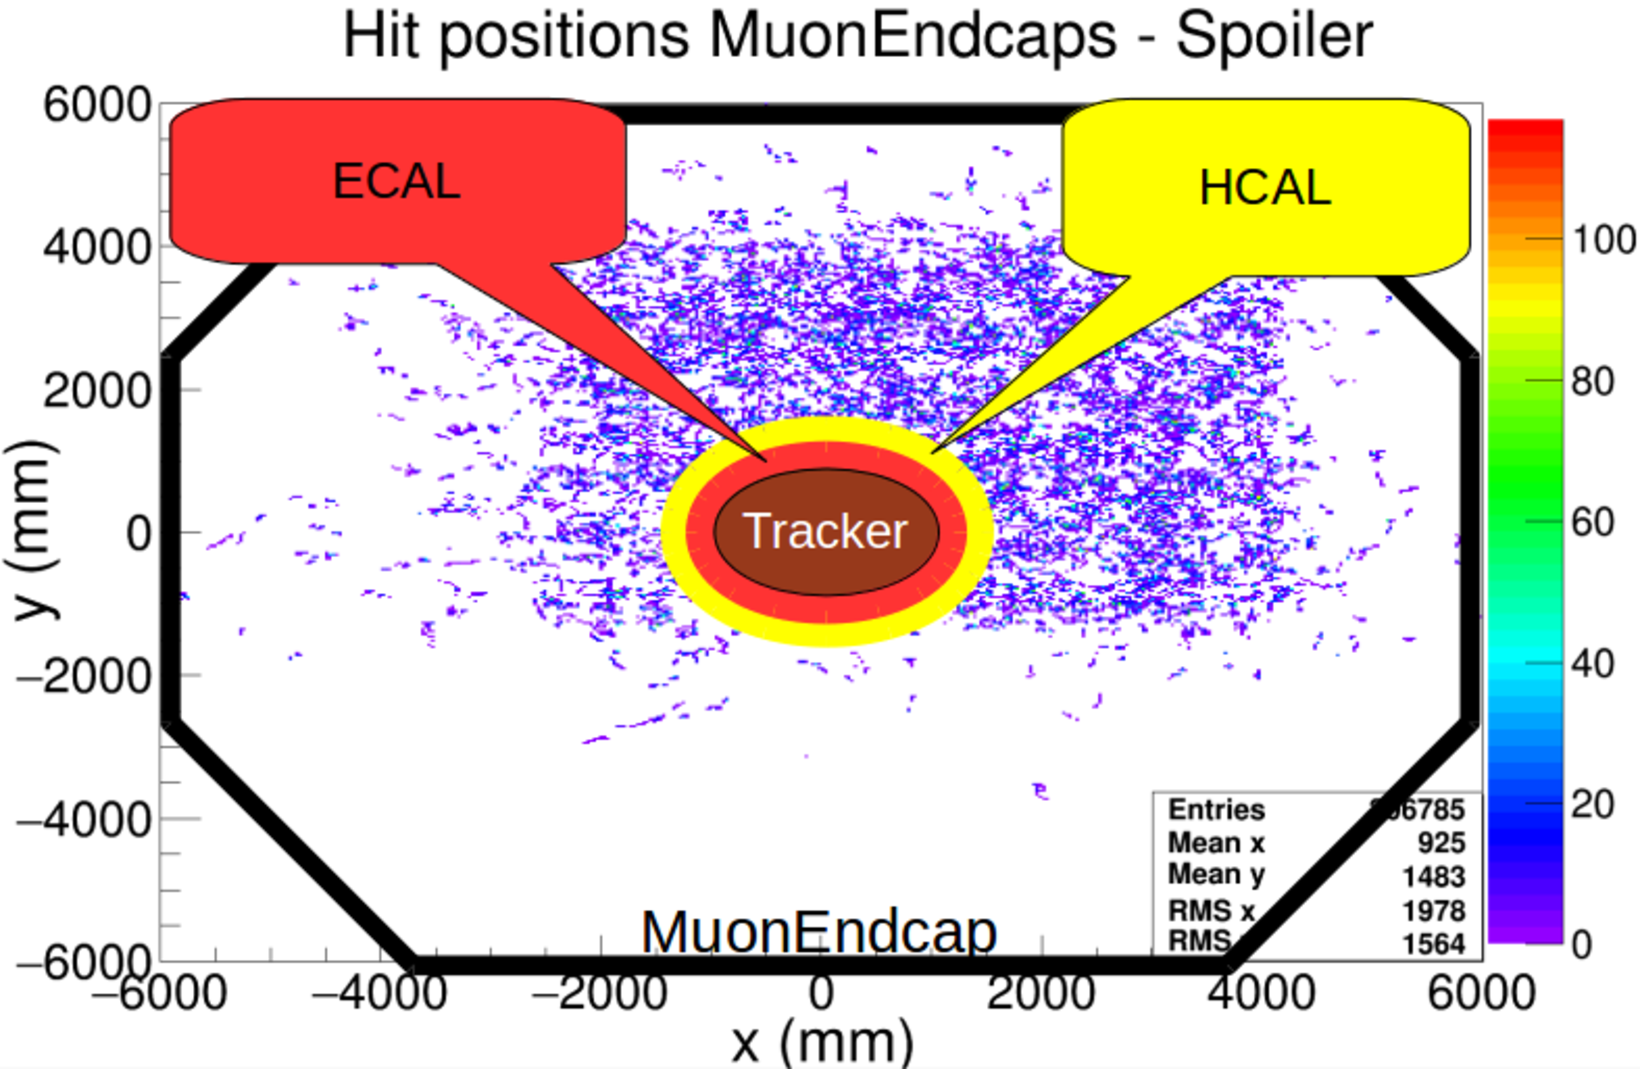
\includegraphics[width=0.45\textwidth]{figures/Explanation_Hits_Subdetectors.pdf}\\
The number of hits in the different SiD subdetectors for both shielding scenarios (\textcolor{Red}{``5 Spoilers''} and \textcolor{Blue}{``5 Spoilers + Wall''}) is not evenly distributed.\\
The number of hits depends on the effective area of the subdetector system.
 \end{frame}
 
\begin{frame}{The Muon Energy}
\begin{center}
  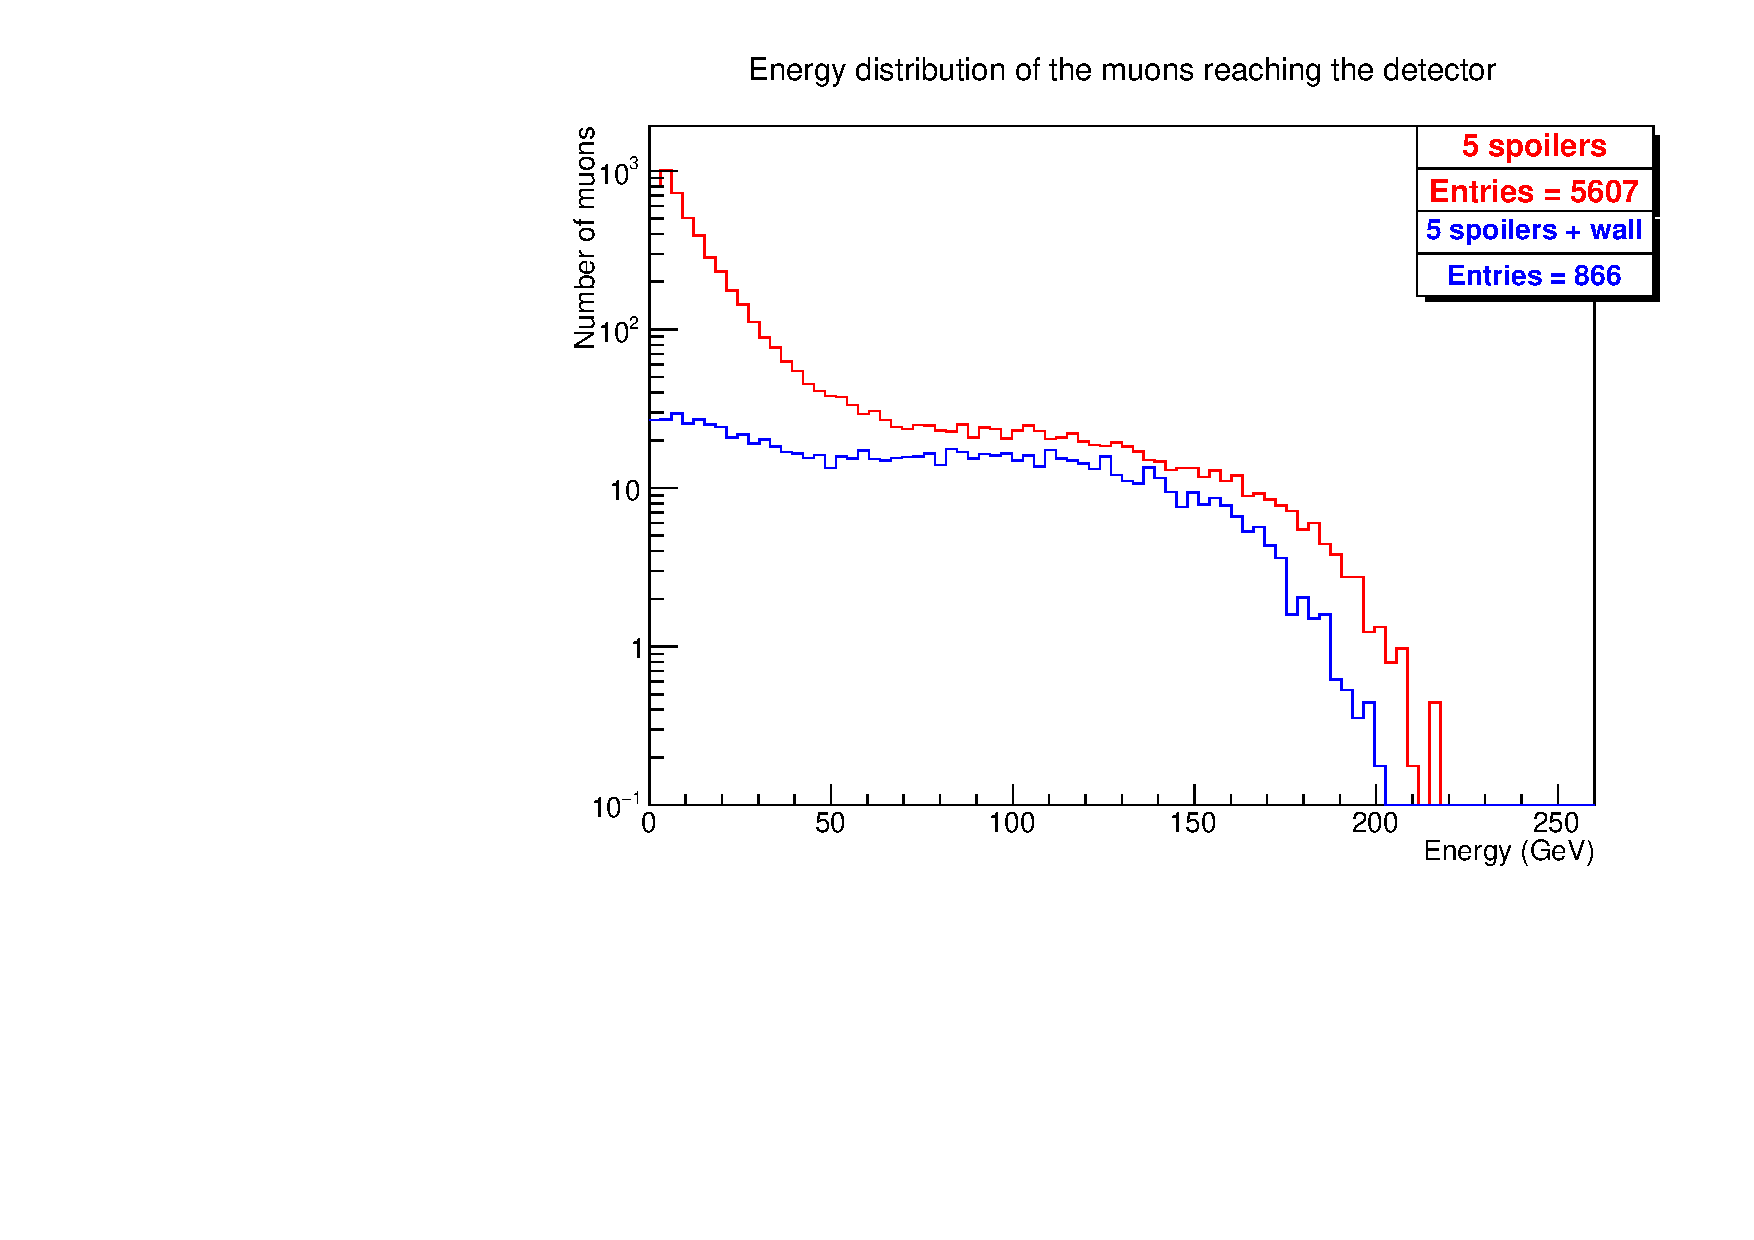
\includegraphics[width=0.65\textwidth]{figures/muon_energy.pdf}
\end{center}
The energy distribution of the muons from the ``5 Spoilers + Wall'' scenario does not reach the same maximum energy. The muons are decelerated and stopped within the magnetized wall.
\end{frame}

\end{document}
